\makeatletter
\makeatother
\documentclass[10pt,english]{article}\usepackage{graphicx, color}
%% maxwidth is the original width if it is less than linewidth
%% otherwise use linewidth (to make sure the graphics do not exceed the margin)
\usepackage{alltt}
\usepackage[T1]{fontenc}
\usepackage[latin9]{inputenc}
\usepackage{geometry}
\geometry{left=1.5cm,right=1.5cm,top=2cm,bottom=2cm}
\usepackage{fancyhdr}
\pagestyle{fancy}
\setlength{\parskip}{\smallskipamount}
\setlength{\parindent}{0pt}
\usepackage{amsthm}
\usepackage{amsmath}
\usepackage{subfigure}

\makeatletter

%%%%%%%%%%%%%%%%%%%%%%%%%%%%%% LyX specific LaTeX commands.
\providecommand{\LyX}{L\kern-.1667em\lower.25em\hbox{Y}\kern-.125emX\@}

%%%%%%%%%%%%%%%%%%%%%%%%%%%%%% Textclass specific LaTeX commands.
\numberwithin{equation}{section}
\numberwithin{figure}{section}

\@ifundefined{date}{}{\date{}}
%%%%%%%%%%%%%%%%%%%%%%%%%%%%%% User specified LaTeX commands.
\pagestyle{empty} 

\makeatother

\usepackage{babel}
\begin{document}

\title{Week5 Report}


\author{Xiaohui Li, Yuxin Ma}

\maketitle


This week we mainly focus on two parts based on the contents of the meeting last week. First, we want to find the power curve pattern when units $N$ is increased. Next, turning from 'sparse effects' to 'dense effects',  we analyze the high-dimensional $Y$'s effect upon power.

\section{Units $N$ Analysis}
We want to find that if we increase the units number $N$, how the power pattern will change. We use $N=100$ to $N=1,000,000$ increased by 10 times every time. Also, we fix K, $r_1=\frac{Y_1}{\sigma_1}$ and $r_k=\frac{\sigma_k}{\sigma_1}$ this time where $Y_1$ varies from 0 to 1, and do the same test for minimum, median and mean value for the $p_{combined}$.
\begin{figure}[htbp]
\centering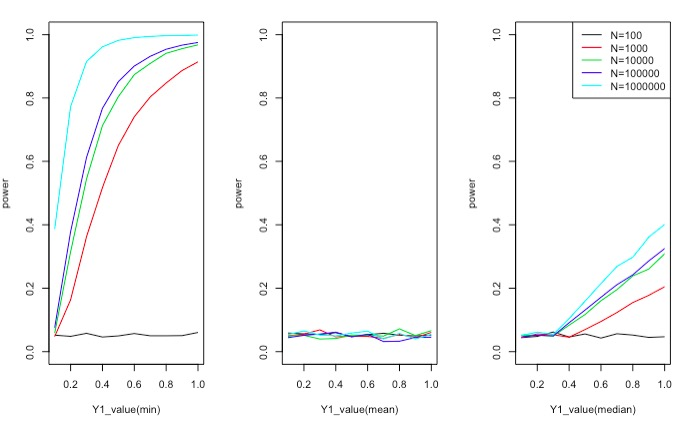
\includegraphics[width=8in, height=4in]{N}
\caption{Units $N$ analysis}
\end{figure}
\quad\\
From the plot we can see that, the median and mean perform not well under this condition. So for the minimum, as $N$ increases, the power will converge to 1 faster.

\section{High-dimensional Analysis}
\subsection{Power Analysis}
For the further discuss, we do not only vary $Y_1$ for the treatment. Except fixing $Y_0=0$, we vary all the rest $Y$ by multivariable normal distribution this time. We use the 'mvtnorm' package in \textbf{R} to generate $Y$, and since we control $||Y||=\epsilon$, we further generate $Y_{norm}=\frac{Y}{\sqrt{\sum Y^2}}\cdot\epsilon$.\\
\quad\\
For the test, we control all $\sigma=1$ and vary $\epsilon$ from 0 to 1 to compute the power. To get more information, we also do the same test for minimum, median and mean value for the p\_combined. Meanwhile, we try different units number $N$ as well.\\
\subsubsection{Test of power variation}
As a pretest we test for the variation of power given fixed epsilon norm but random direction level $\vec{Y}$, we assigned the $\epsilon$ with value 0.1.\\
\begin{figure}[htbp]
\centering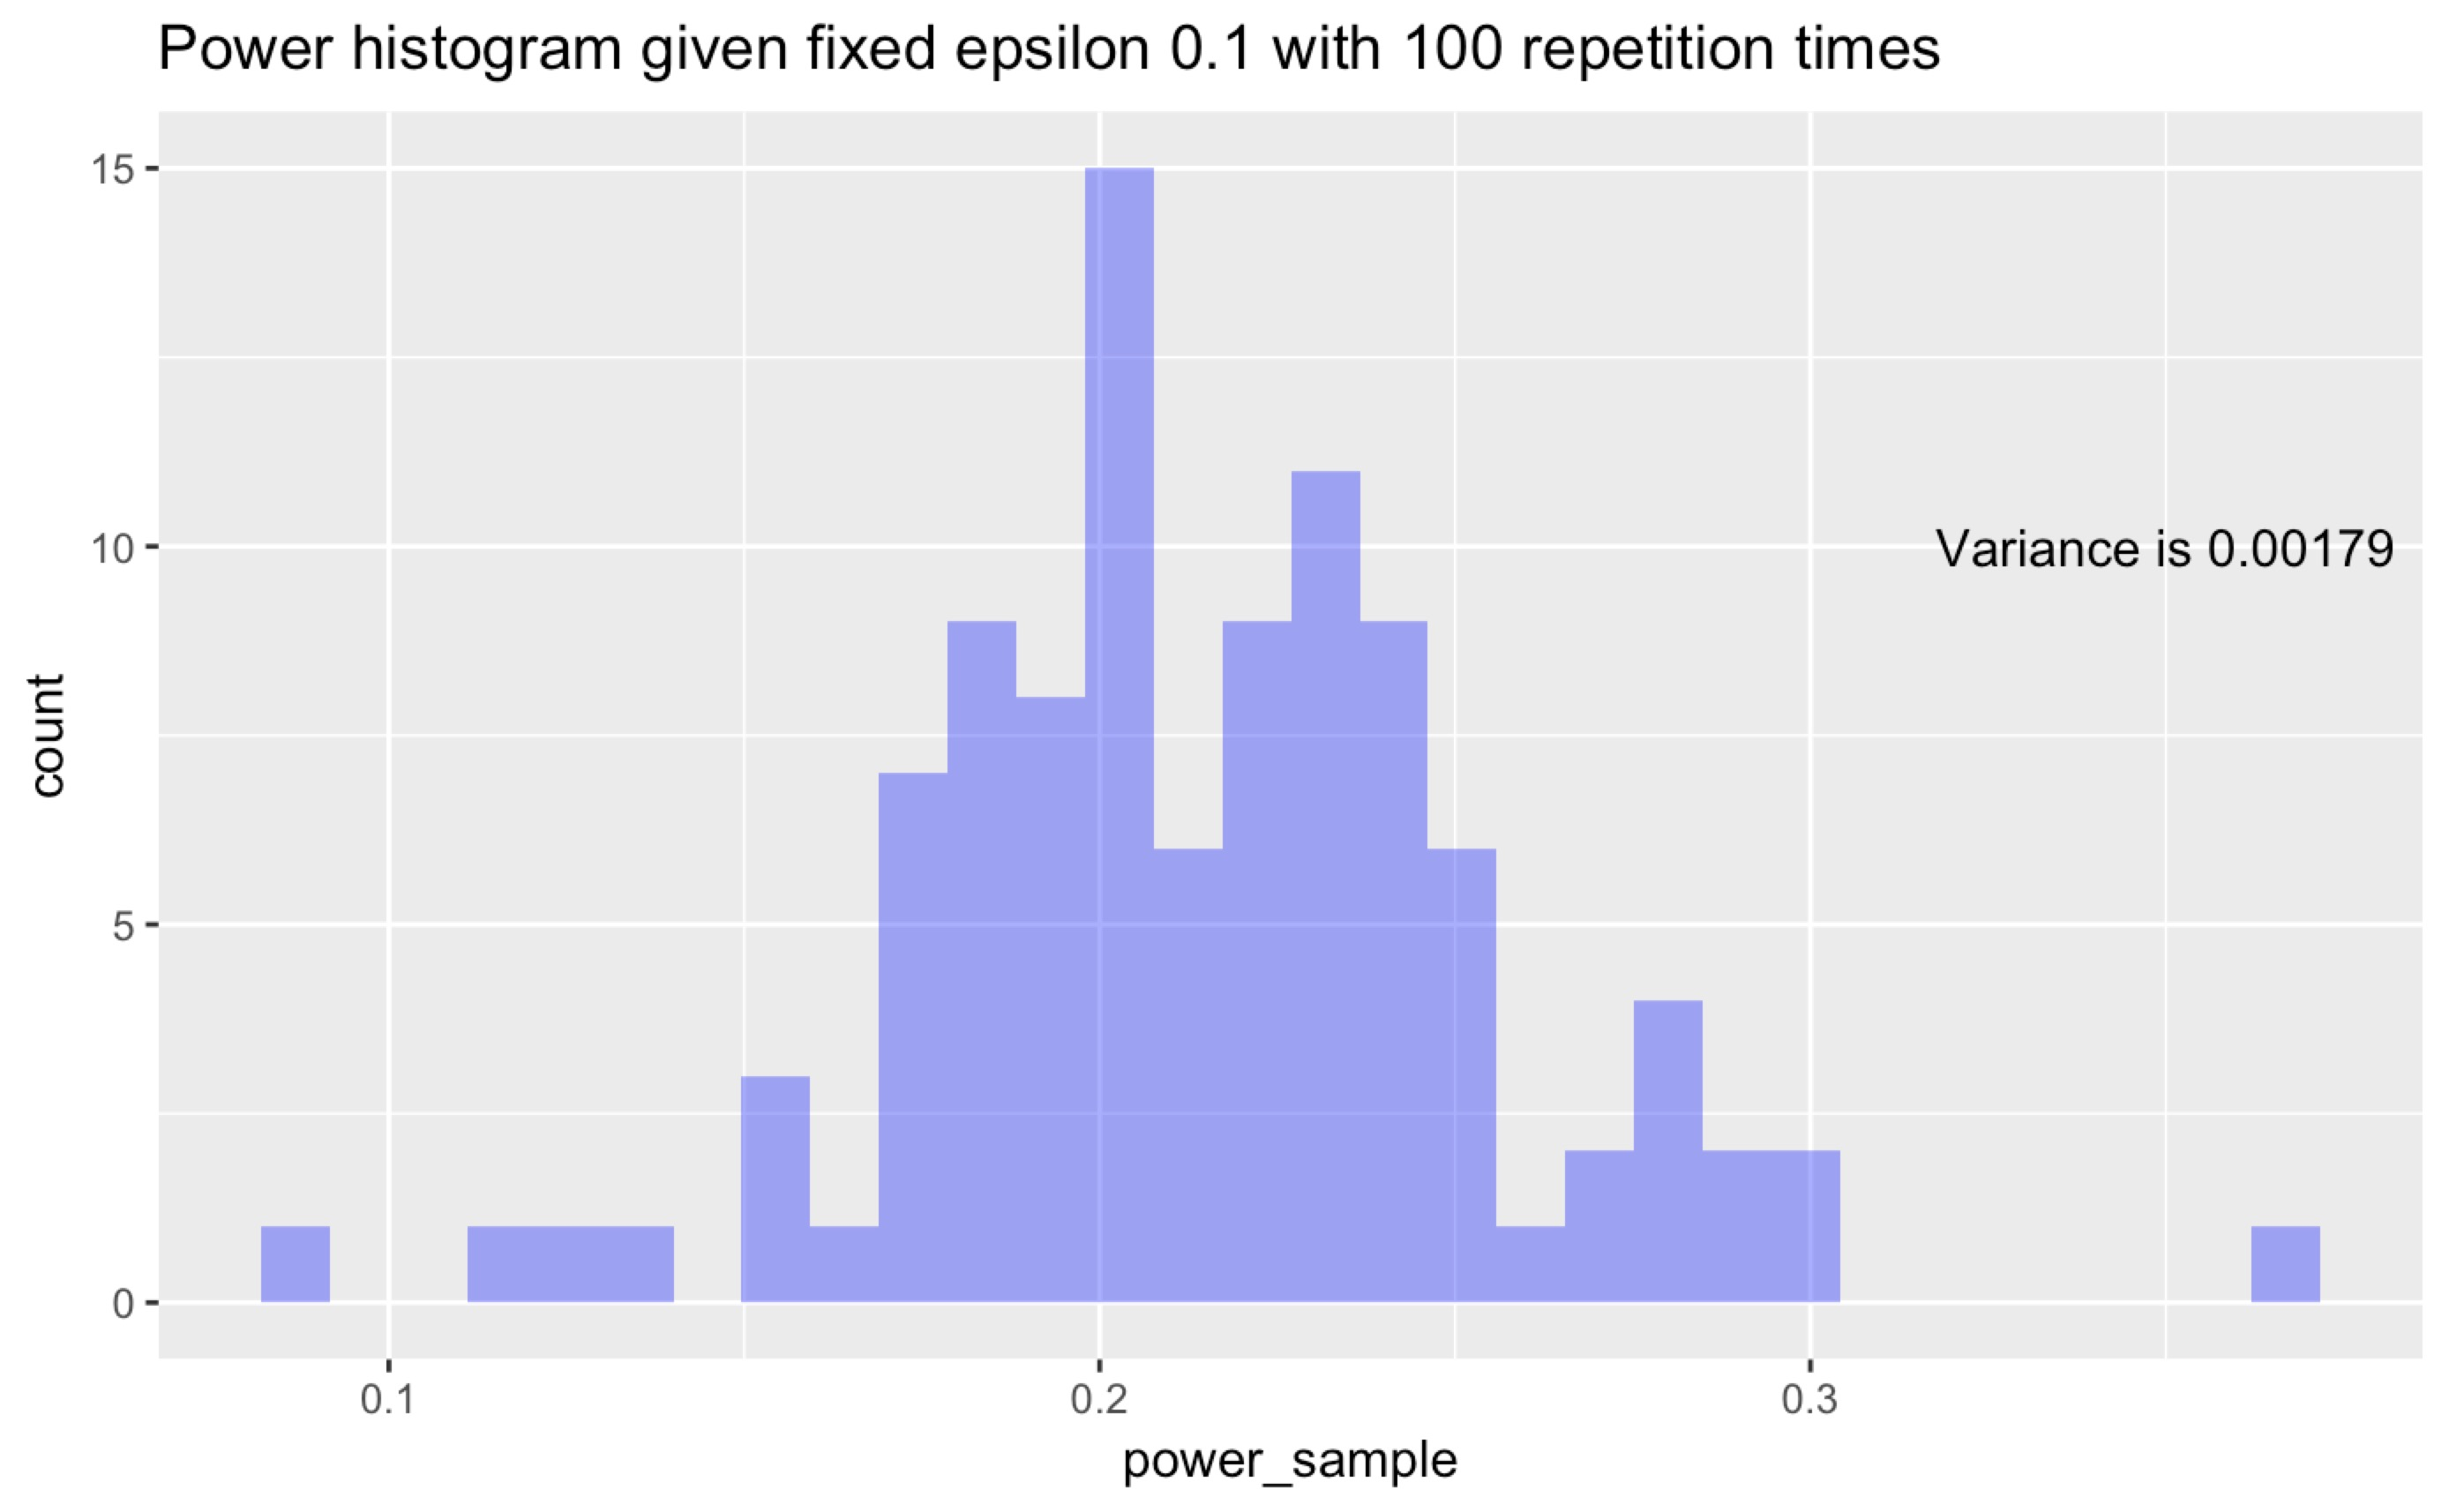
\includegraphics[width=4.5in, height=3in]{histo}
\caption{Histogram of Power given fixed epsilon}
\end{figure}
\quad\\
We find that as repetition times increase the sample variance gets less and the mean is more , from pre test, 100 reptition times is accurate enough.
\newpage
\subsubsection{Power curve}
The power curves respectively for \textbf{minimum}, \textbf{median} and \textbf{maximum} are shown below.
\begin{figure}[htbp]
\centering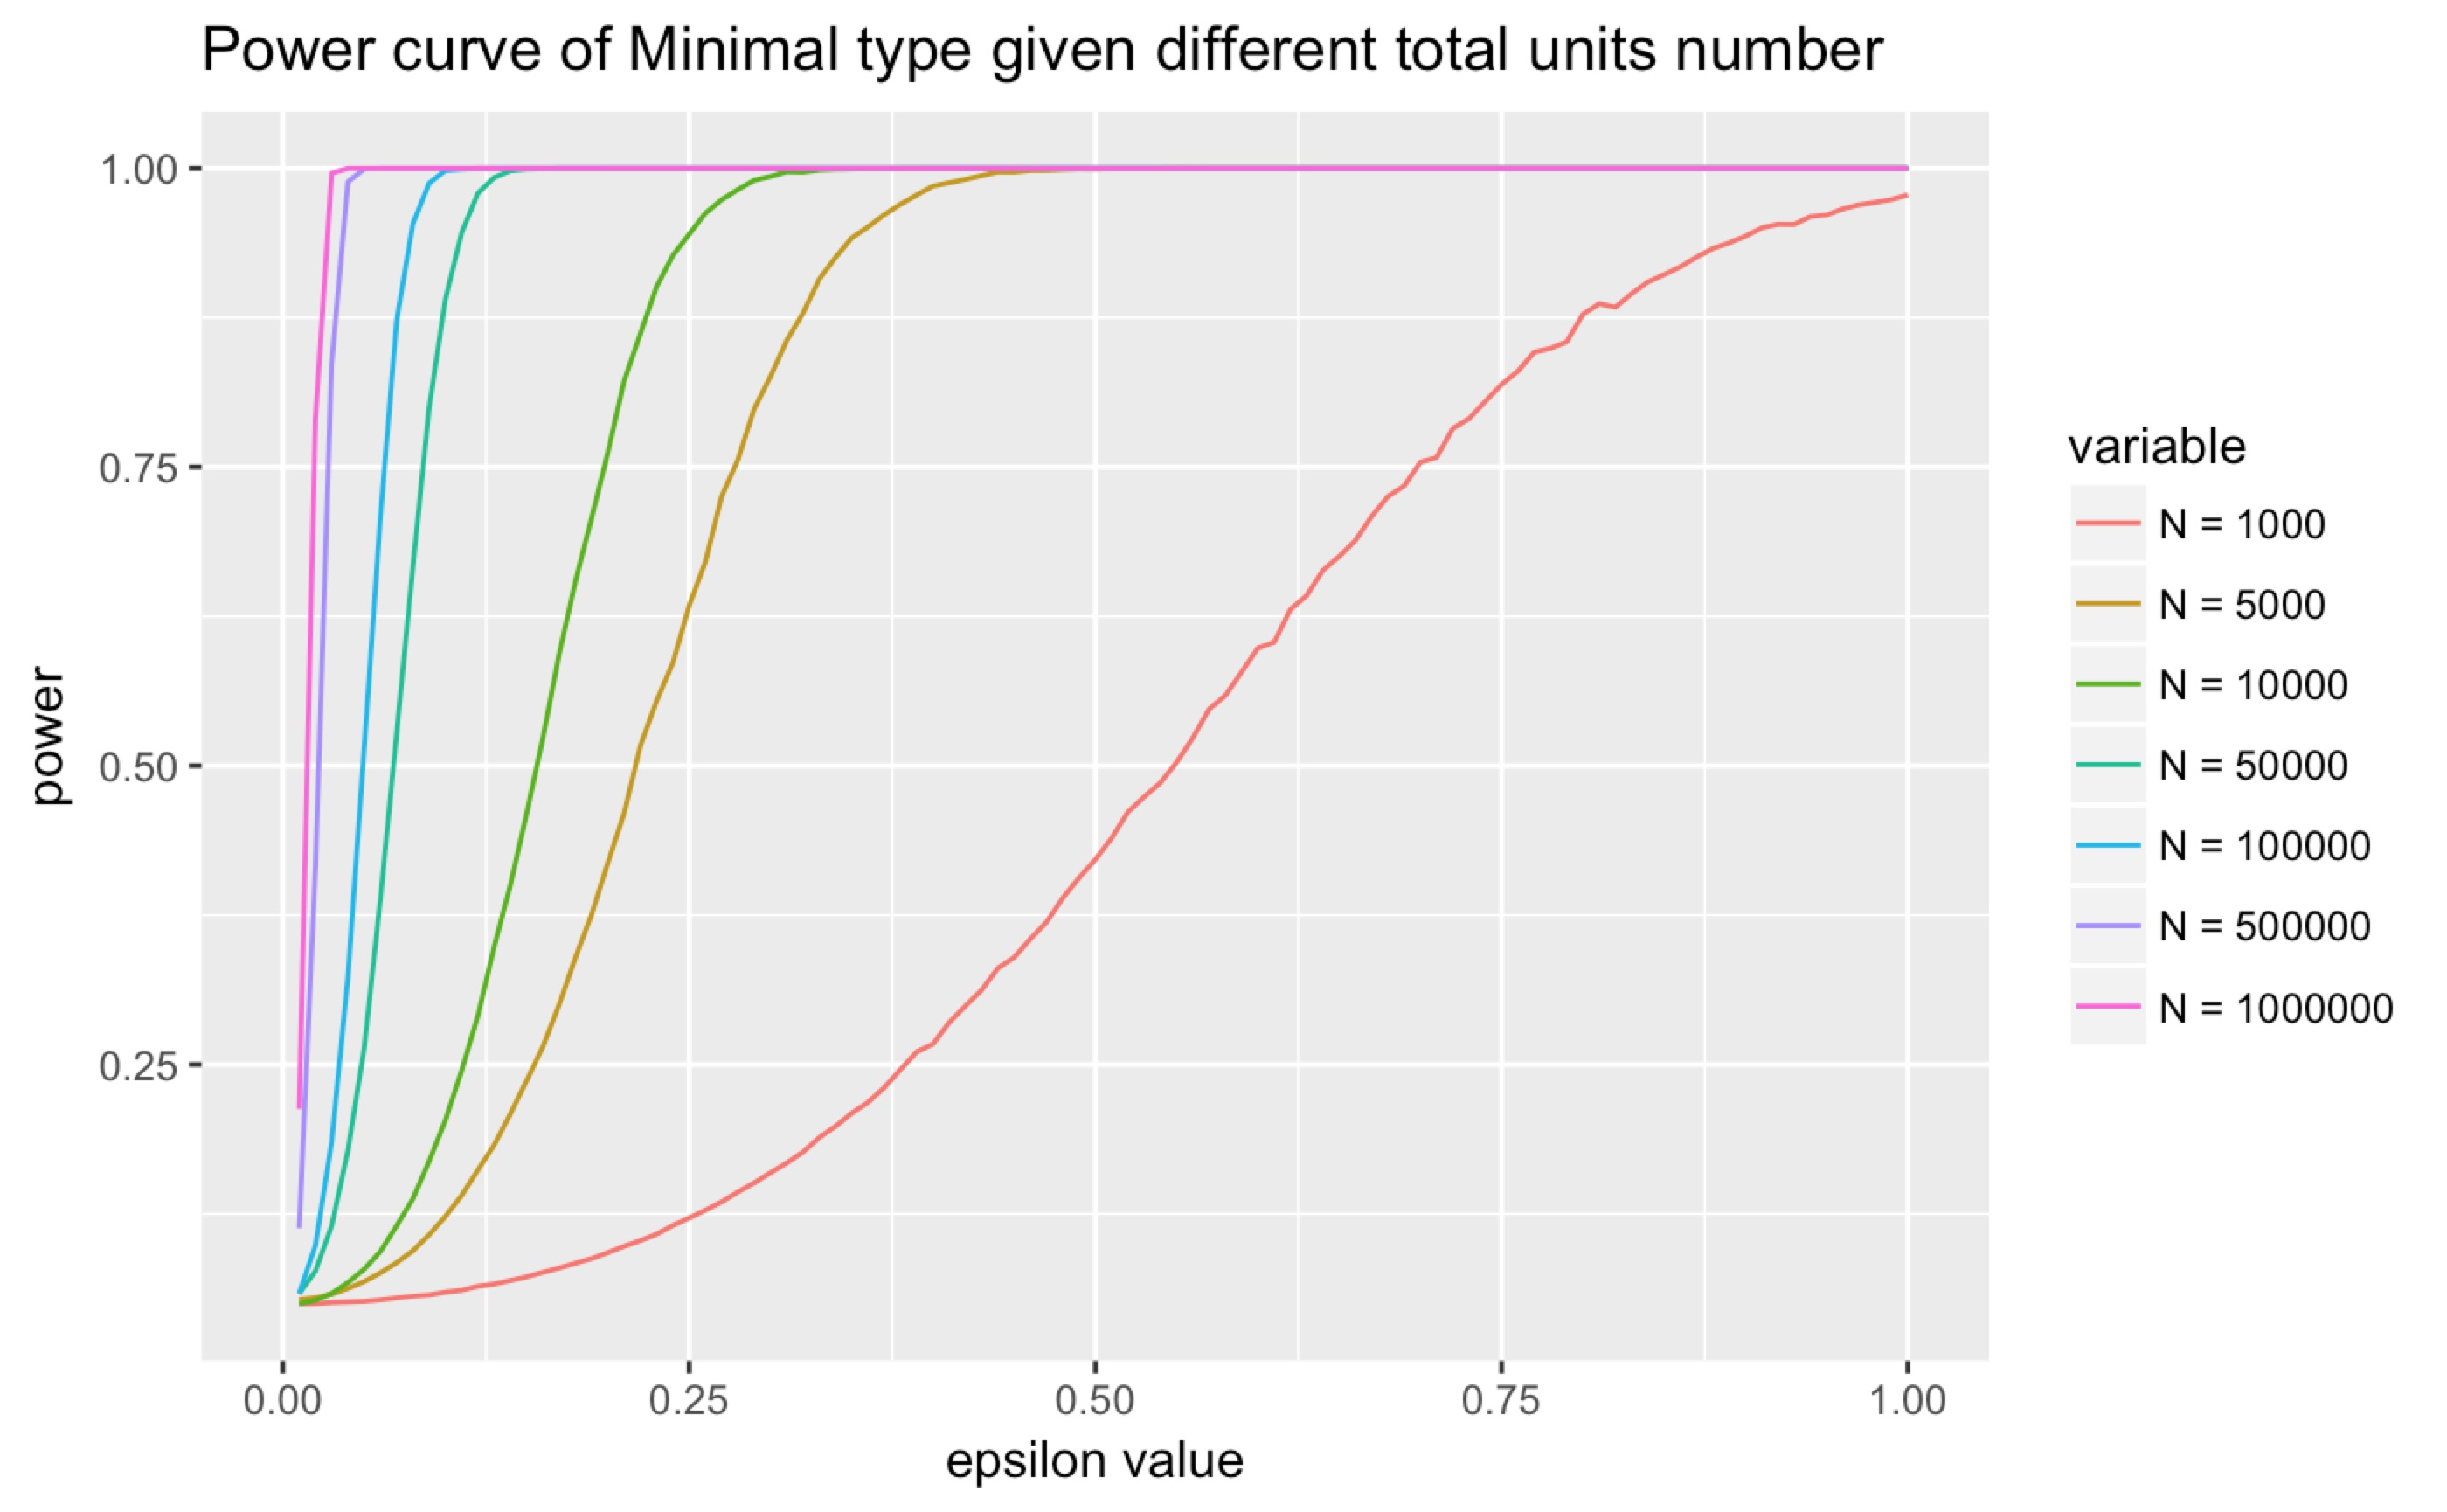
\includegraphics[width=4.5in, height=3in]{min}
\caption{High-dimensional analysis for minimum}
\end{figure}
\begin{figure}[htbp]
\centering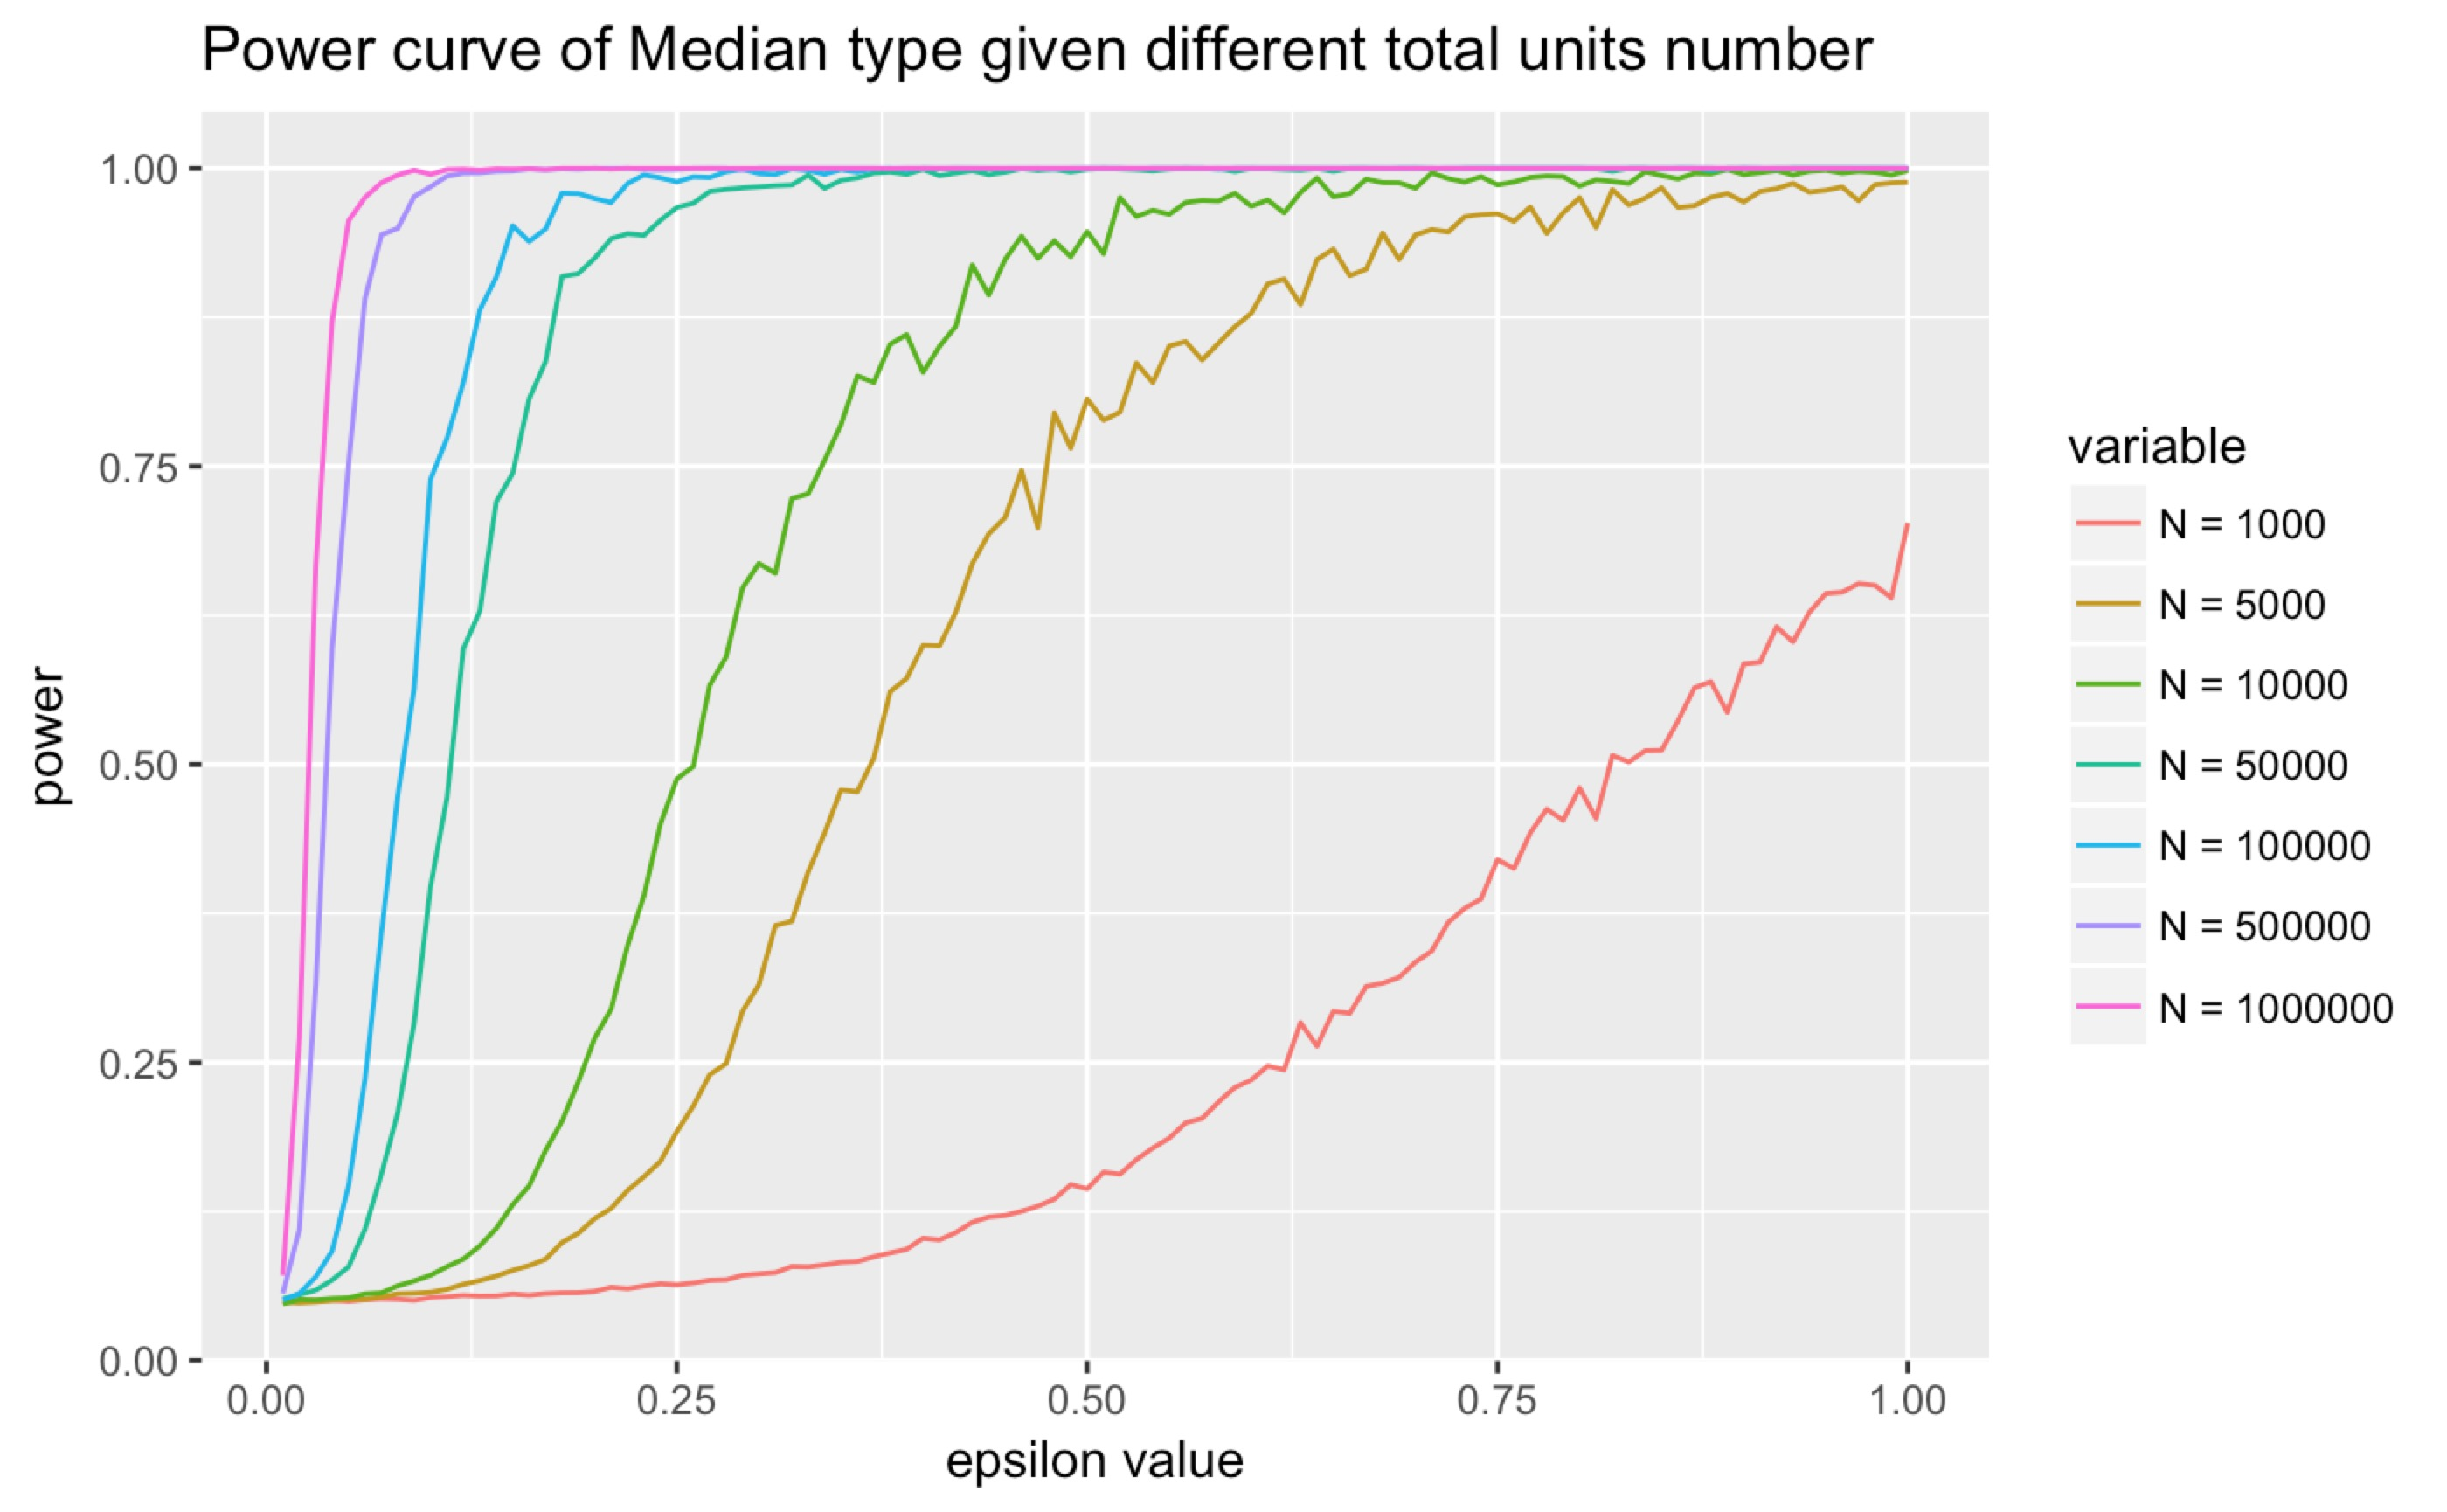
\includegraphics[width=4.5in, height=3in]{median}
\caption{High-dimensional analysis for median}
\end{figure}
\newpage
\begin{figure}[htbp]
\centering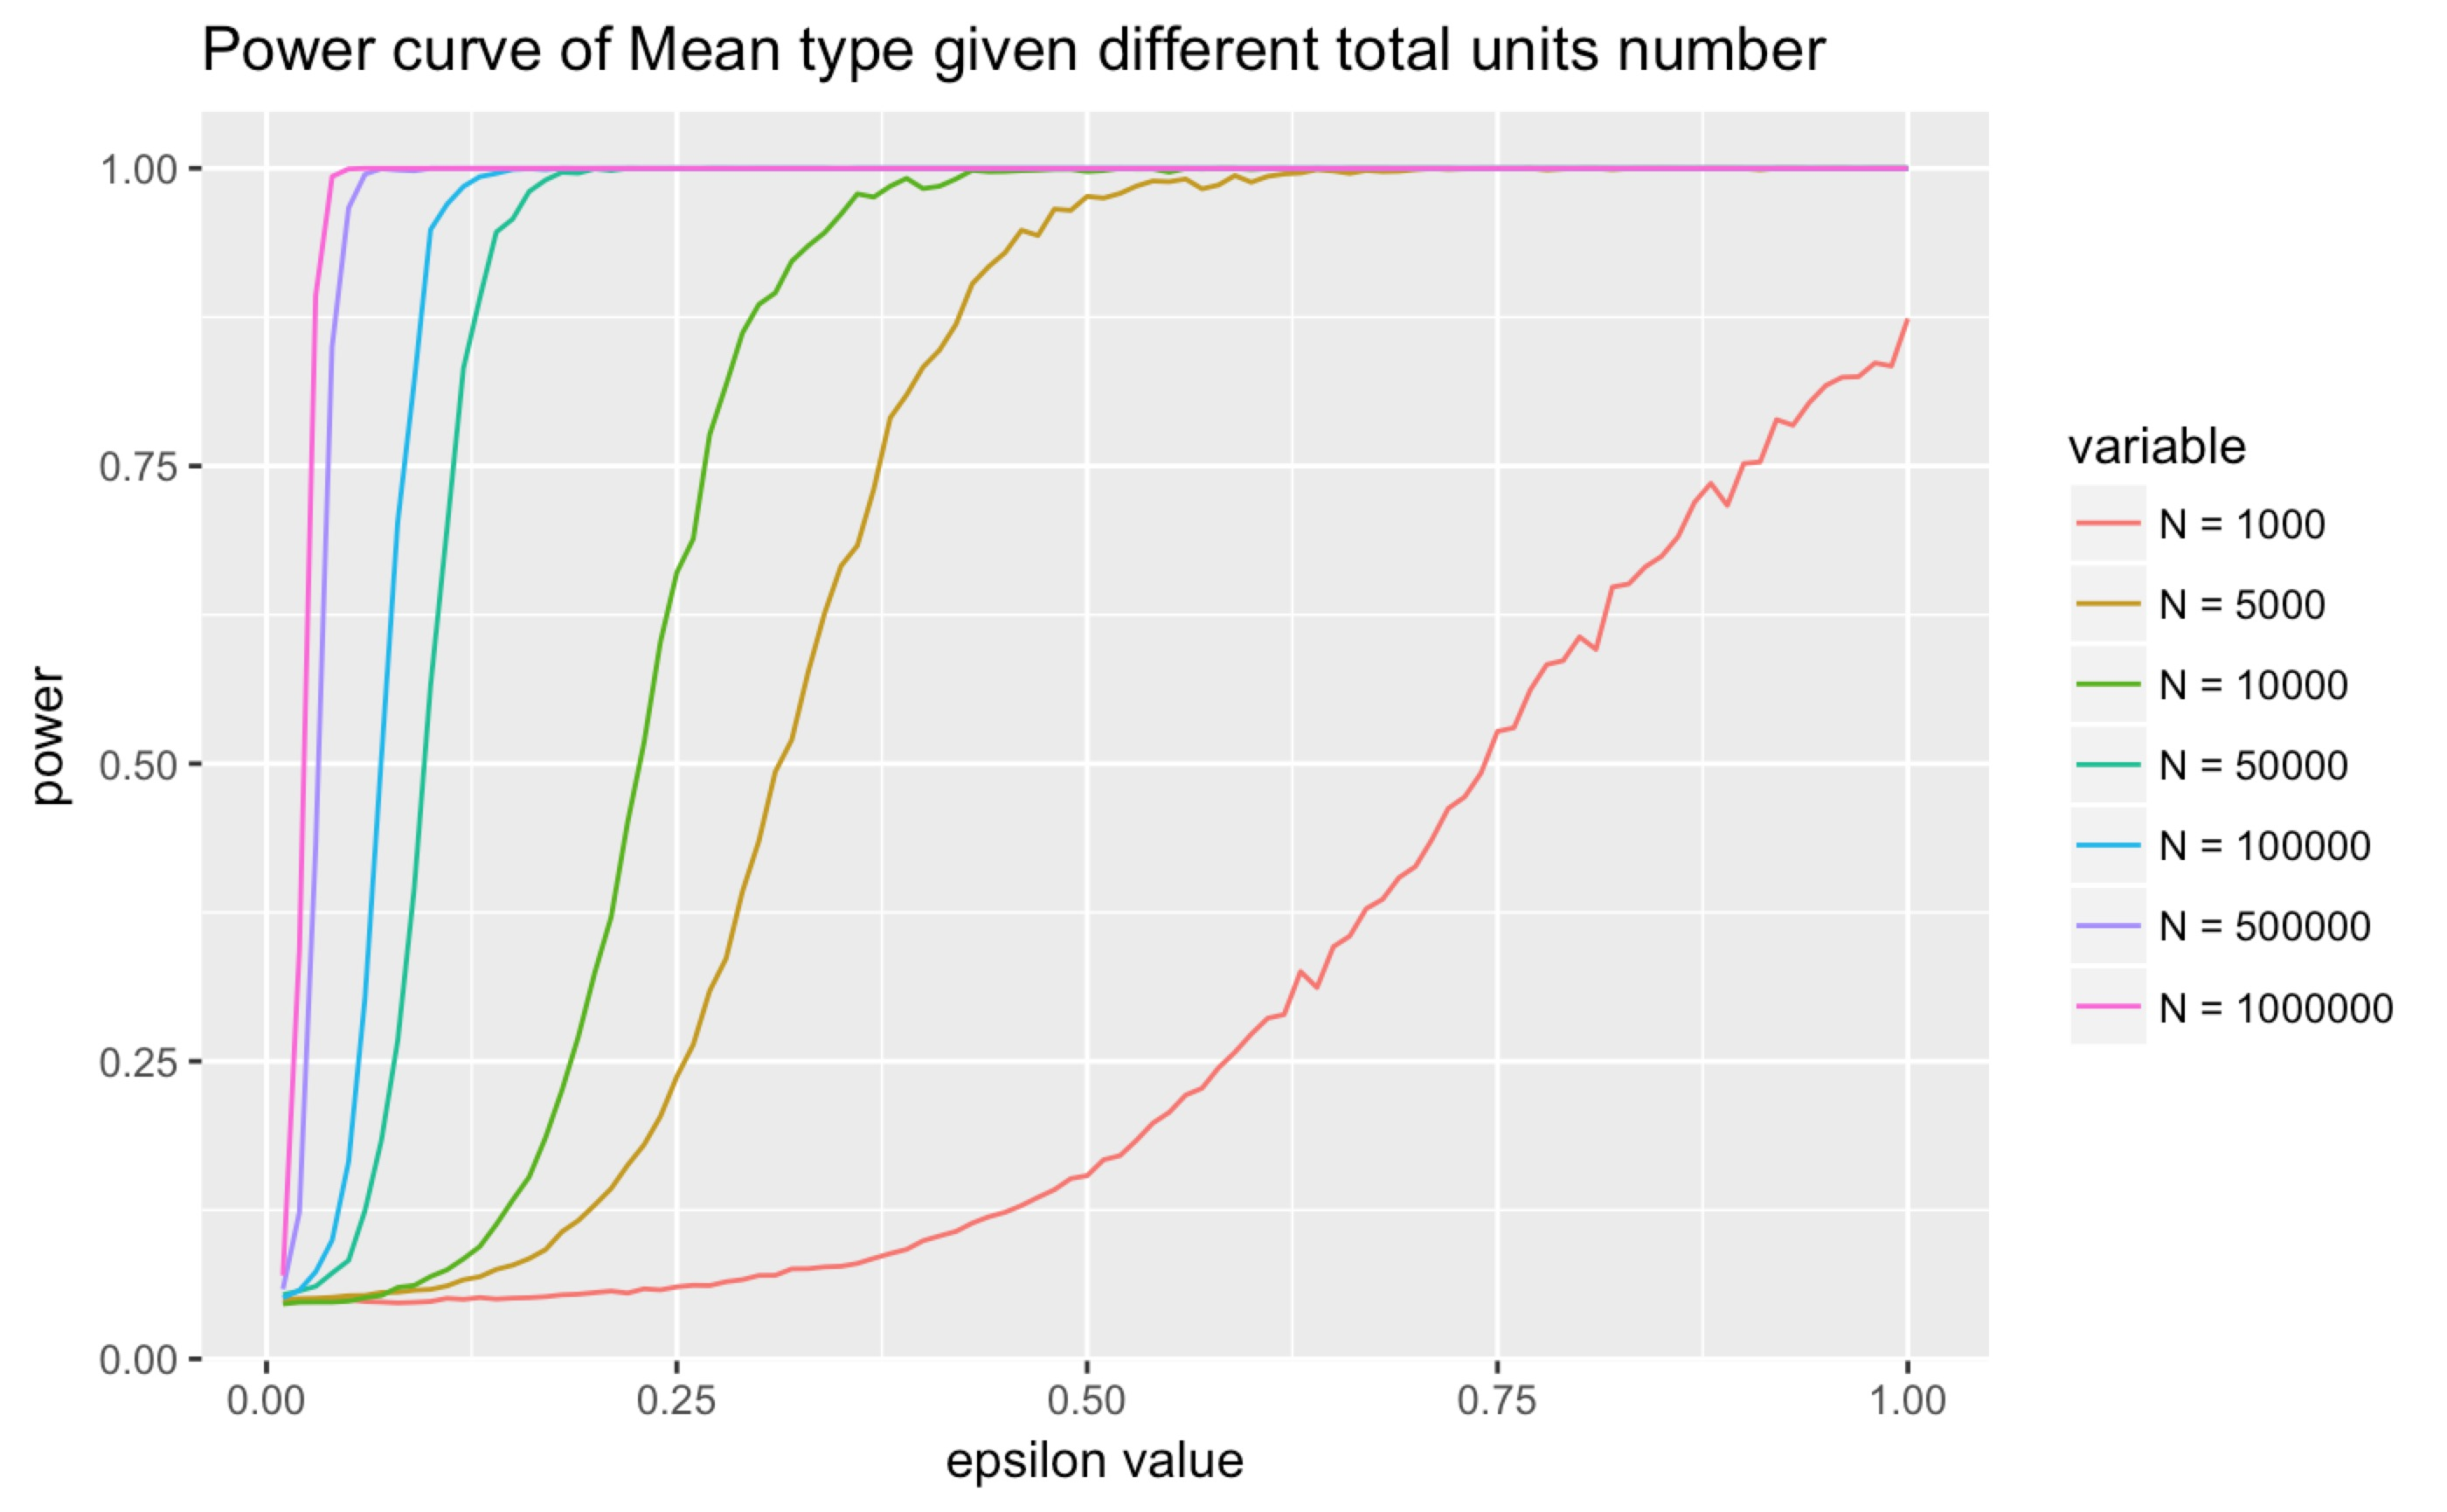
\includegraphics[width=4.5in, height=3in]{mean}
\caption{High-dimensional analysis for mean}
\end{figure}
\quad\\
We can see that the units number $N$ has the same trend as before: the larger $N$, the faster the speed at which the power converges to 1. But unlike in the single normal distribution, 1-dimensional analysis before, all three plots perform pretty well under the high-dimensional analysis. But the minimum seems to be smoother and more stable than the other two. And mean is better than median.\\
\newpage
\subsection{Critical Epsilon Analysis}
We generate a new 80\% power critical epsilon function with binary algorithm. And we fix the N to be 10000 and vary the K from 2 to 100 to see the relationship between critical epsilon and K.\\

\begin{figure}[htbp]
\centering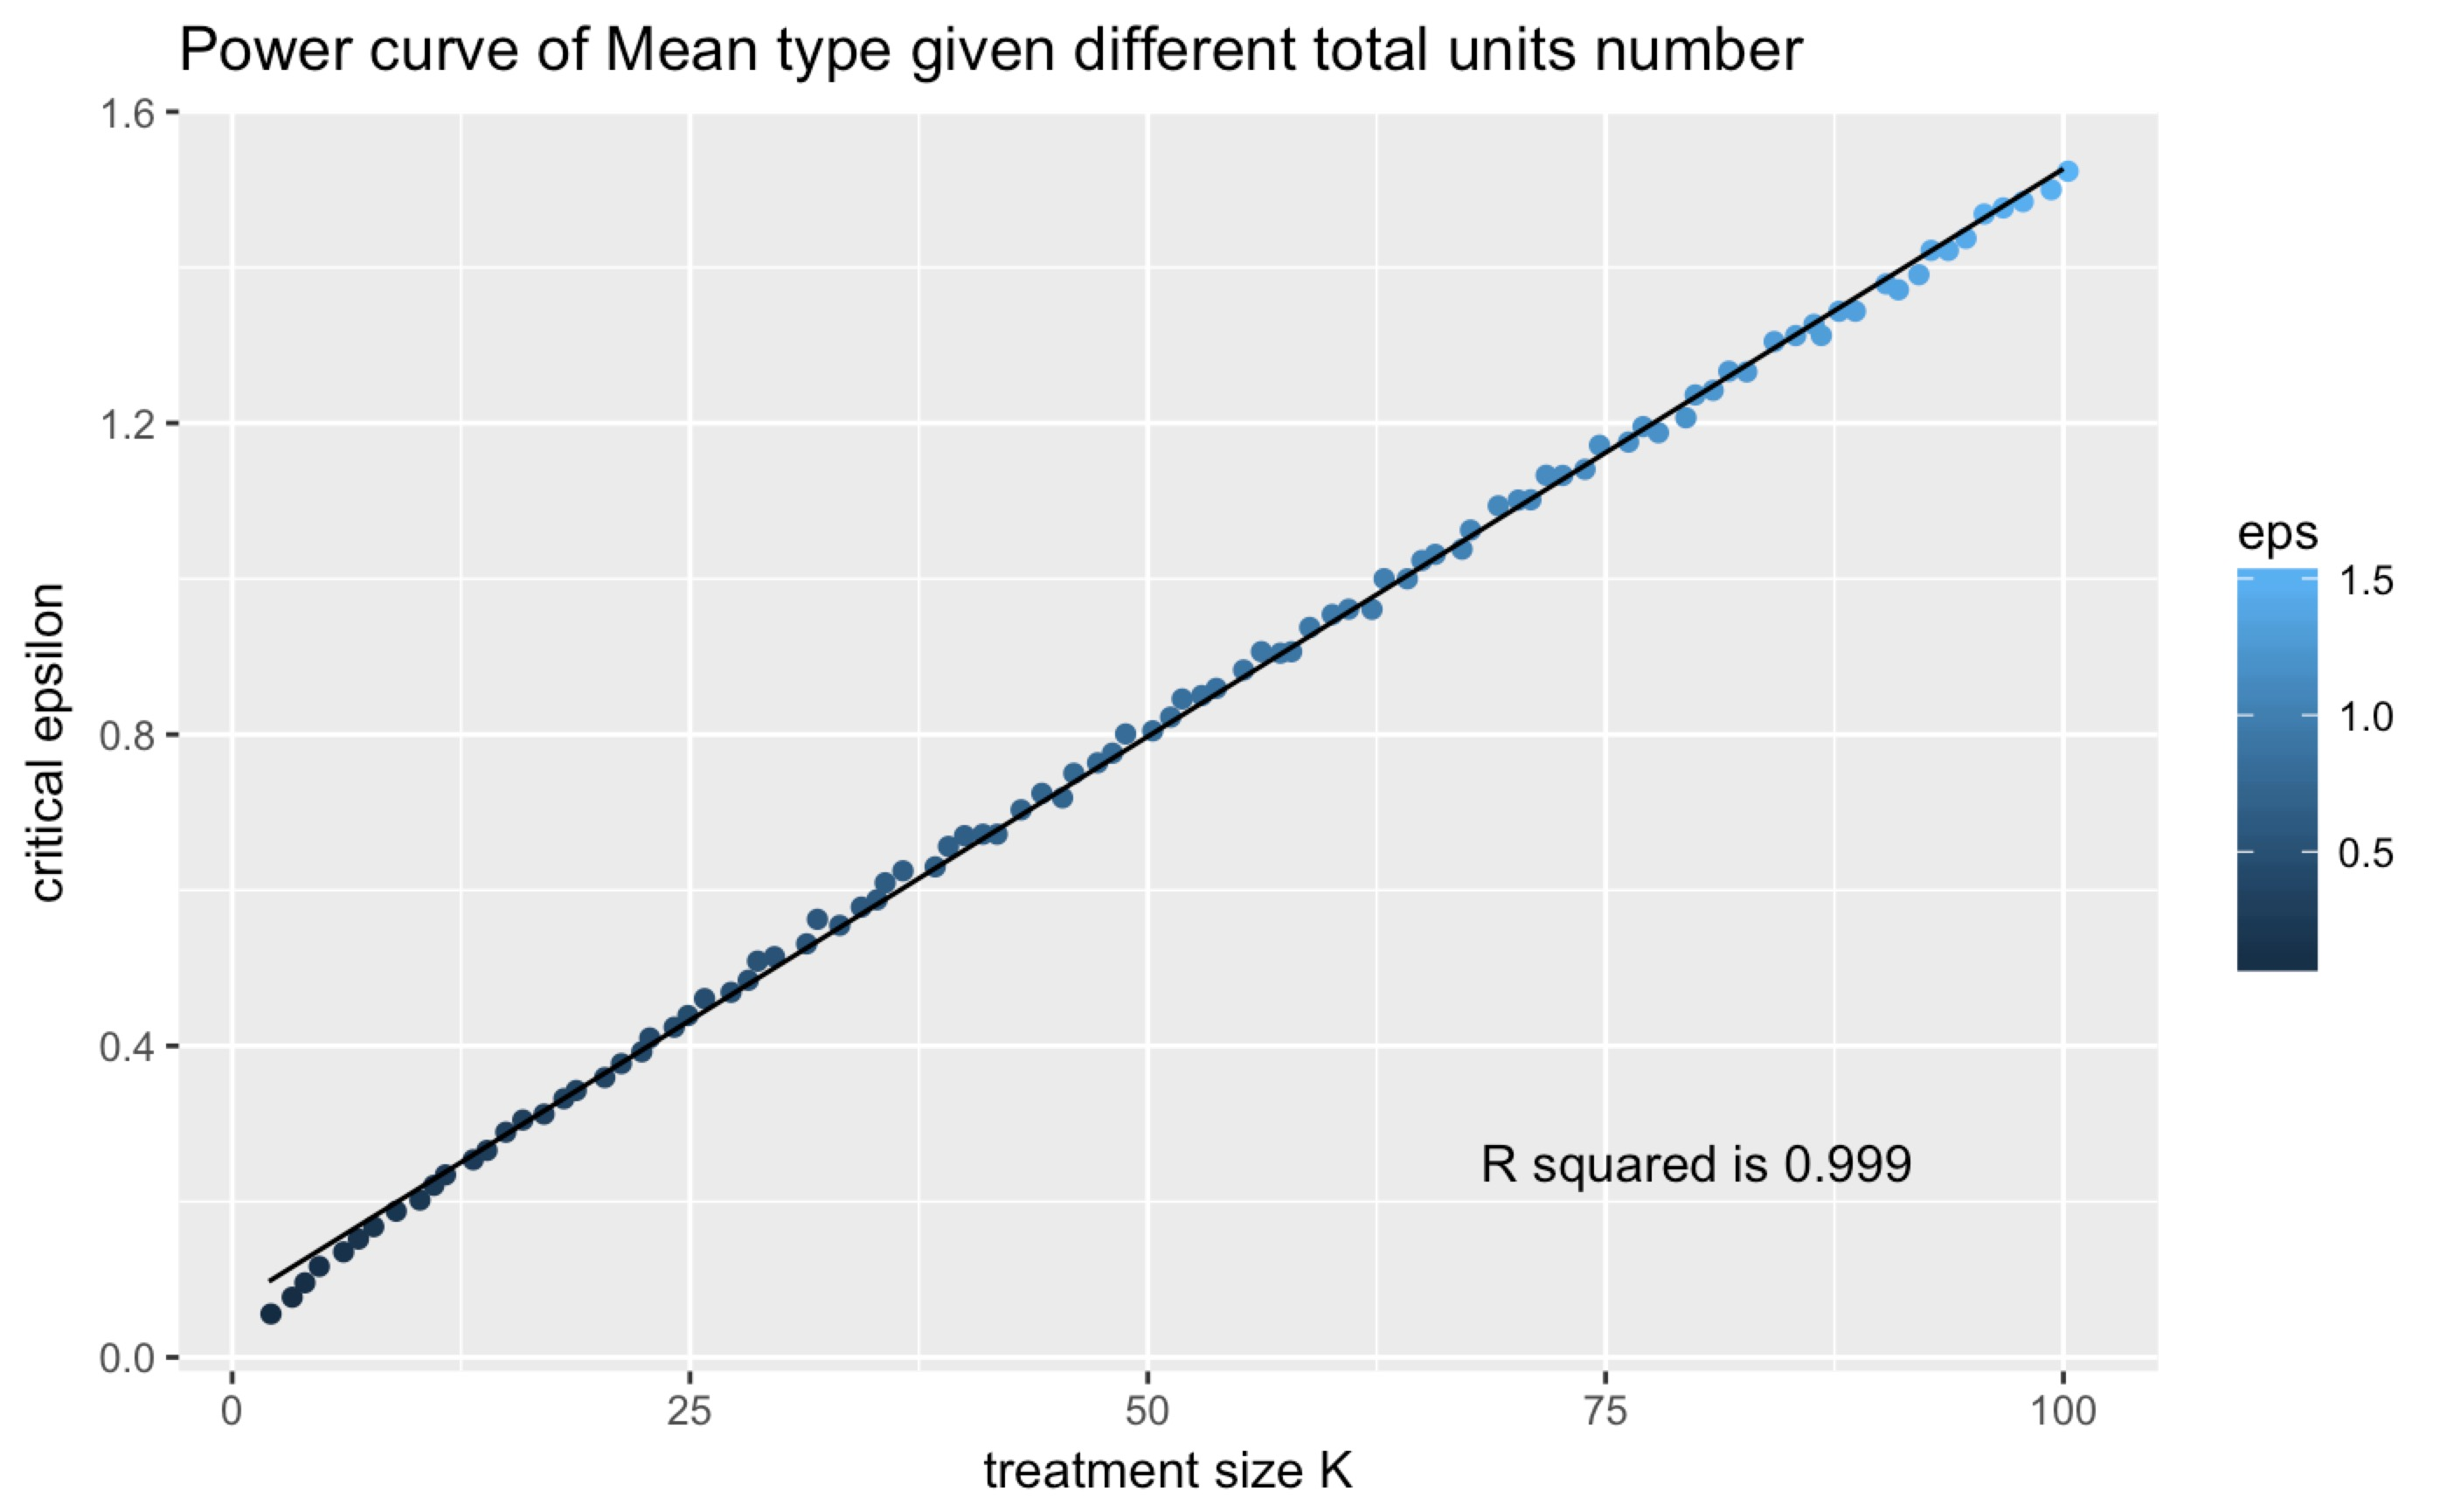
\includegraphics[width=6in, height=4in]{epsilon}
\caption{Critical epsilon analysis for treatment size K}
\end{figure}

\begin{figure}[htbp]
\centering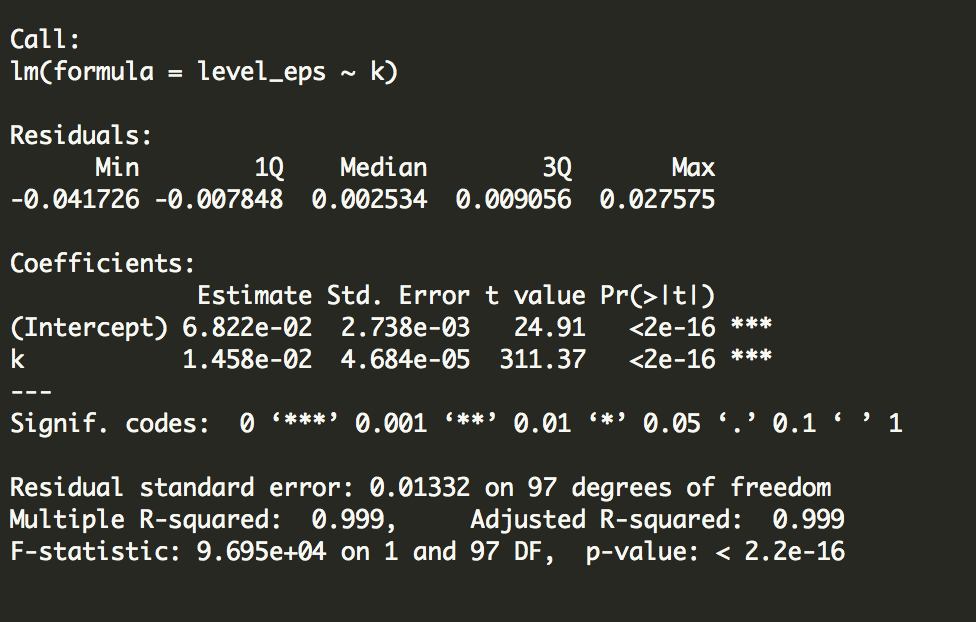
\includegraphics[width=4in, height=2in]{reg}
\caption{Linear regression summary of Epsilon against treatment K}
\end{figure}

We find that the critical epsilon is linearly increasing along with K and the R squared is enormously large as 0.999, suggesting theoretical linear model. 
$\epsilon_{\{ P(Y_{\epsilon})  \quad\\ = \quad\\  0.8)\}} = 1.48K$

\end{document}










